% \documentclass[handout]{beamer}
\documentclass{beamer}
\usepackage[ruled,linesnumbered]{algorithm2e}
\usepackage{natbib}
%\usepackage{enumitem}
\definecolor{vuborange}{rgb}{1.0,0.40,0.0}
\usetheme{Boadilla}
\usepackage{booktabs}
\title{Efficiently Explaining CSPs with Unsatisfiable Subset Optimization}
\institute[shortinst]
{\inst{1} Vrije Universiteit Brussel, Belgium \\ % Your institution for the title page
\inst{2} KULeuven, Belgium \\ % Your institution for the title page
\href{mailto:emilio.gamba@vub.be}{\underline{emilio.gamba@vub.be}}, \href{mailto:bart.bogaerts@vub.be}{bart.bogaerts@vub.be}, \href{mailto:tias.guns@kuleuven.be}{tias.guns@kuleuven.be} % Your email address
}
\date{IJCAI 2021}

\author{\underline{Emilio Gamba}\inst{1} \and  Bart Bogaerts\inst{1} \and   Tias Guns\inst{1,2}}

\newcommand\m[1]{\ensuremath{#1}\xspace}
\newcommand\allconstraints{\m{T_P}}
\newcommand\formula{\ensuremath{\m{F} }\xspace}
\newcommand\formulac{\ensuremath{\m{C} }\xspace}

\makeatletter
\setbeamertemplate{footline}
{
  \leavevmode%
  \hbox{%
  \begin{beamercolorbox}[wd=.2\paperwidth,ht=2.25ex,dp=1ex,center]{author in head/foot}%
    \usebeamerfont{author in head/foot}Emilio Gamba (VUB)
  \end{beamercolorbox}%
  \begin{beamercolorbox}[wd=.6\paperwidth,ht=2.25ex,dp=1ex,center]{title in head/foot}%
    \usebeamerfont{title in head/foot}Efficiently Explaining CSPs with Unsatisfiable Subset Optimization
  \end{beamercolorbox}%
  \begin{beamercolorbox}[wd=.2\paperwidth,ht=2.25ex,dp=1ex,right]{date in head/foot}%
    \usebeamerfont{date in head/foot}August 2021\hspace*{1em}
    \insertframenumber{} / \inserttotalframenumber\hspace*{2ex} 
  \end{beamercolorbox}}%
  \vskip0pt%
}
\makeatother

\begin{document}

\begin{frame}
    \maketitle
\end{frame}


\begin{frame}
	\frametitle{Outline}

	\begin{enumerate}
		\item Motivation
		\begin{itemize}
			\item Explanations for logic puzzles (but also for CSPs)
			\item Generating an explanation sequence for CSPs
		\end{itemize}
		\item Contributions and Applicability
		\begin{enumerate}
			\item Optimality \& Constrainedness
			\item Incrementality
		\end{enumerate}
	\item Results
	\item Conclusion
	\item Ideas for future work
	\end{enumerate}
\end{frame}

\begin{frame}{Motivation}
	\framesubtitle{Logic Grid Puzzles}
	\begin{figure}
		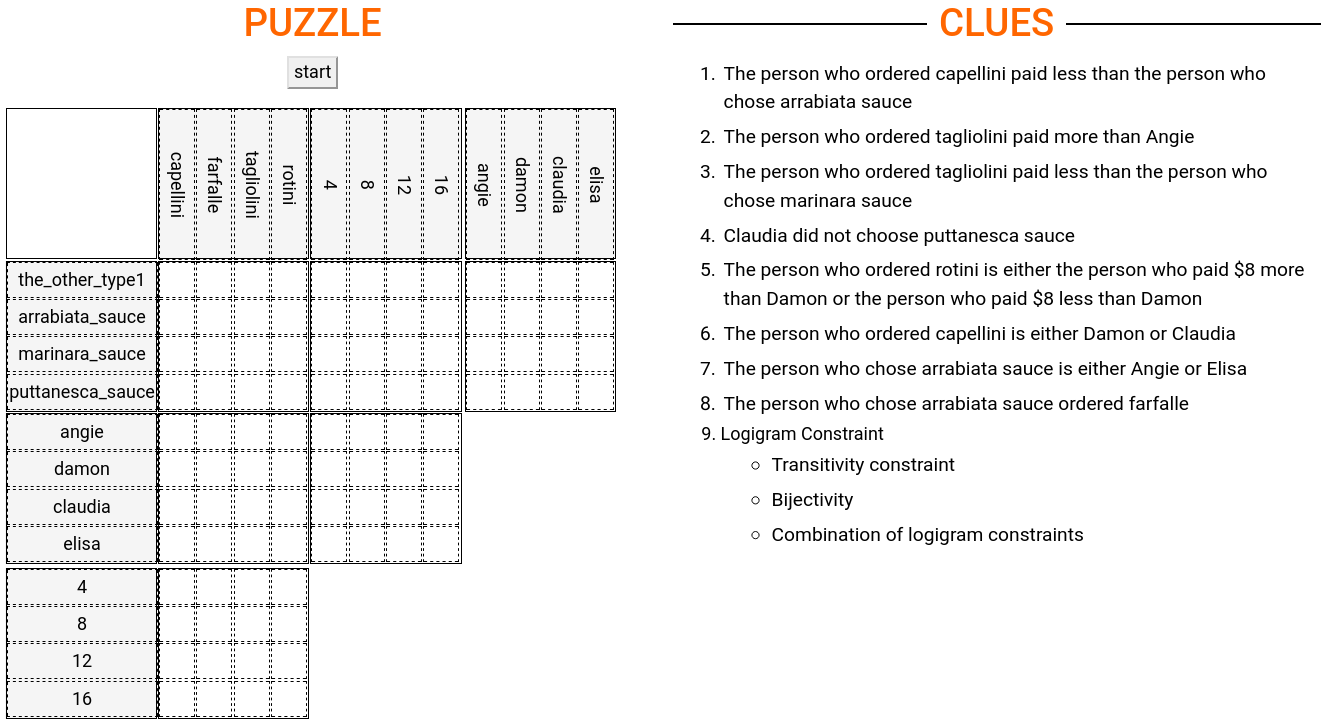
\includegraphics[width=0.9\textwidth]{logicpuzzles.png}
	\end{figure}
\begin{center}
\url{https://bartbog.github.io/zebra/pasta/}
\end{center}
\end{frame}

\begin{frame}{Motivation}
	\framesubtitle{CSPs: a little formal Background}
	
	\begin{itemize}
%		\setlength{\leftmargin}{0pt}
		\item[$\m{C}$] \emph{constraints} we can use to reason (alldifferent, George did not take pasta, …)
		\item[$I_0$] an \emph{Initial Interpretation}
		\item[$I_{end}$] Everything we can derive from $ \m{C} \wedge \m{I}_0$
	\end{itemize}
\begin{figure}
	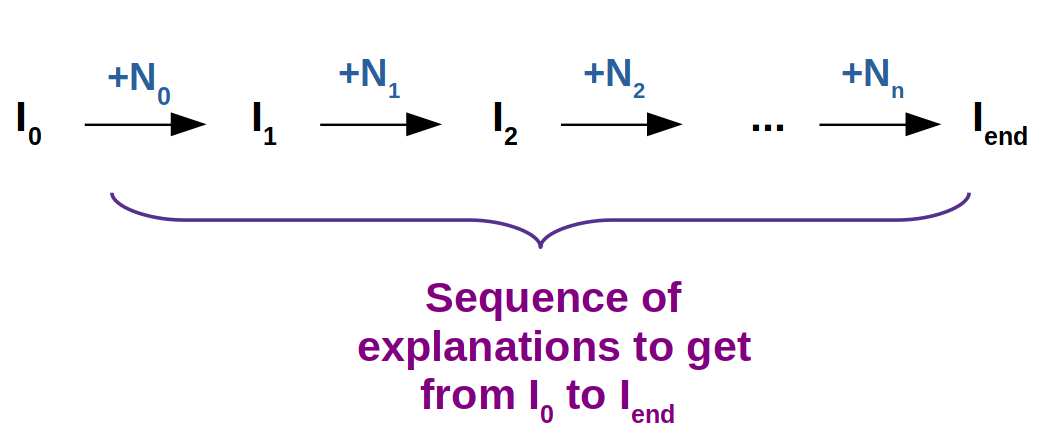
\includegraphics[width=0.7\textwidth]{sequence_explanation.png}
\end{figure}
\end{frame}



\begin{frame}{Motivation}
	\framesubtitle{Gentle reminder: Explanations for CSPs}
	 \begin{definition}
		Given one or a subset of the constraints ( $S_i \subseteq T_P$  ) and facts we know ($E_i\subseteq I_i$), an \textbf{explanation} is an implication of the form $E_i \wedge S_i  \implies N_i $, where $N_i$ is the new information from $S_i \cup E_i \models N_i$.
	\end{definition}

An \textbf{explanation sequence} is of the form $$<(I_0,(\emptyset,\emptyset,\emptyset)),\text{\hspace{3pt}}(I_1,(E_1, S_1, N_1)),\text{\hspace{3pt}}...,\text{\hspace{3pt}}(I_{end},(E_{n}, S_n, N_n ))>$$

\begin{figure}
	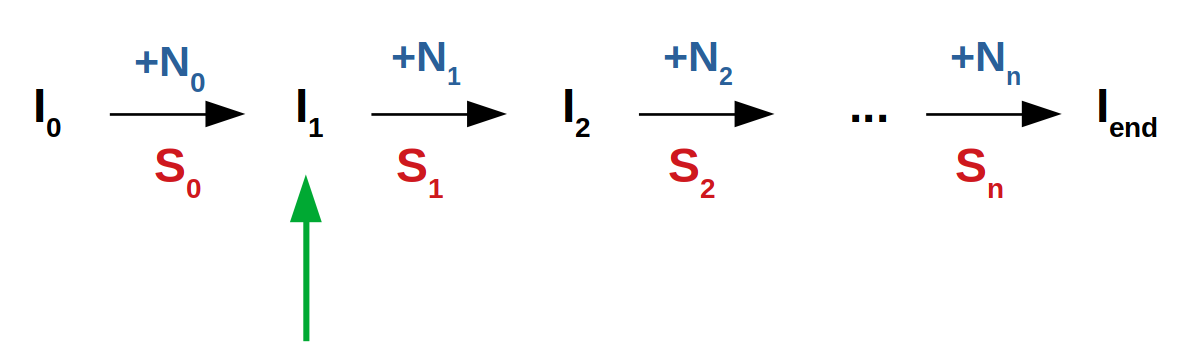
\includegraphics[width=0.7\textwidth]{sequence_explanation2.png}
\end{figure}


\end{frame}

\begin{frame}{Motivation}
		\begin{figure}
		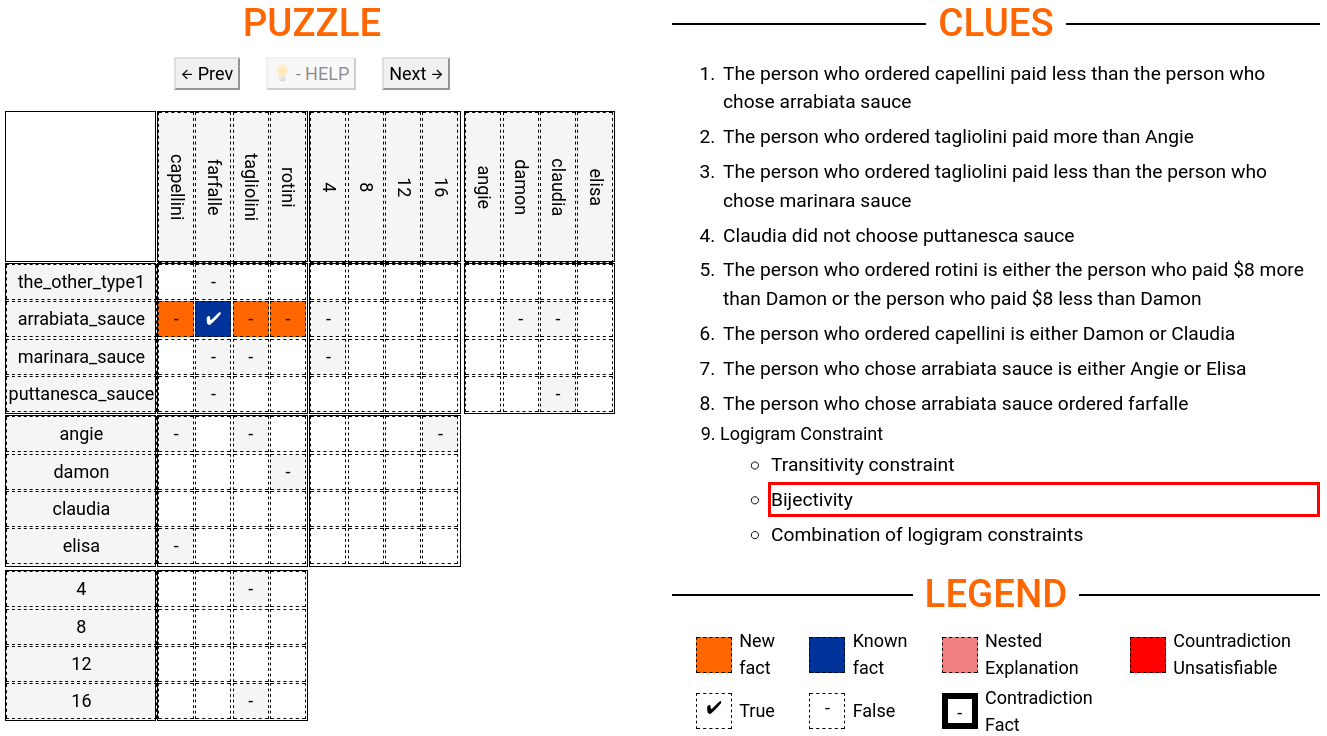
\includegraphics[width=0.6\textwidth]{logic_puzzles_bij.png}
	\end{figure}\pause
\begin{itemize}
	\item[$E_i$] farfalle goes with arrabiata sauce \pause
	\item[$S_i$] an entity of type pasta can only be linked to one entity of type sauce\pause
	\item[$N_i$] taglioni, rotini and capellini cannot be linked to arriabiata
\end{itemize}

\end{frame}

\newcommand\onestep{\ensuremath{\call{explain-One-Step}}\xspace}


\begin{frame}{Motivation}
	\framesubtitle{Generating an explanation sequence for CSPs}
	At every step in the explanation sequence:
	\begin{figure}
		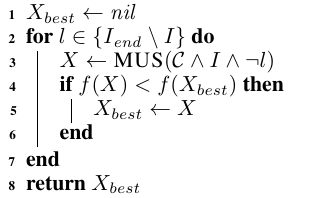
\includegraphics[width=0.45\textwidth]{algo_mus2.png}
	\end{figure}
	 \begin{itemize}
		\item Finding non-redundant explanations: MUS($\formulac \land I \land \neg l$) extraction (IDP system)
		
		\begin{itemize}
			\item In practice, not all constraints at once! 
			\item Consider power sets of constraints sorted by increasing cost
		\end{itemize}
	\end{itemize}
\end{frame}

\begin{frame}{Motivation}
	\framesubtitle{Open Questions}

   \begin{description}[font=\color{vuborange}\itshape]
	\item[\hspace{0.9cm}Optimality] Explanations not optimal, heuristically found \pause
	\item[\hspace{1.05cm}Efficiency] Explanation generation takes a lot of time \pause
	\item[\hspace{0.3cm}Incrementality] Can we reuse information from an explanation call to another? \pause
	\item[Constrainedness] Can we avoid looping over the literals when searching for the next best explanation ?
   \end{description}
\end{frame}

\begin{frame}{Optimality \& Constrainedness}
	\begin{minipage}{0.49\textwidth}
		\begin{itemize}
			\item Inspired by \cite{ignatiev2015smallest}
			\item MIP solver instead of SAT-based
			\item Optimal Hitting set (\emph{\textbf{Optimality}})
		\end{itemize}\pause

	\end{minipage}
	\begin{minipage}{0.5\textwidth}
	\begin{figure}
		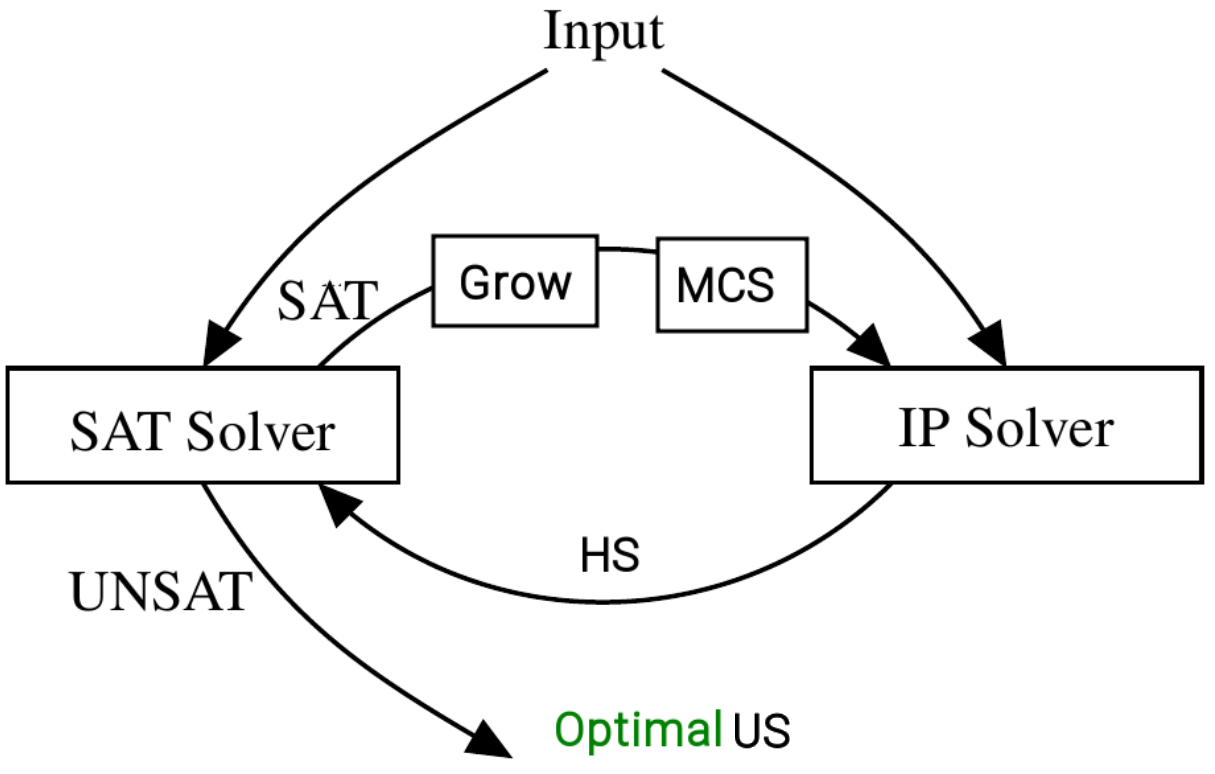
\includegraphics[width=\textwidth]{ihs.png}
\end{figure}
\end{minipage}
\vfill
	\begin{figure}
	
\includegraphics[width=\textwidth]{mus_to_ous.png}
\end{figure}

\end{frame}

\begin{frame}{Optimality \& Constrainedness}
	\begin{minipage}{0.49\textwidth}
		\begin{itemize}
			\item Inspired by \cite{ignatiev2015smallest} with MIP solver
			\item Optimal Hitting set (\emph{\textbf{Optimality}})
			\item 1 literal explained (\emph{\textbf{Constrained}})
		\end{itemize}
	\end{minipage}
	\begin{minipage}{0.5\textwidth}
		% TODO: ADD algorithm  one step !
		\begin{figure}
			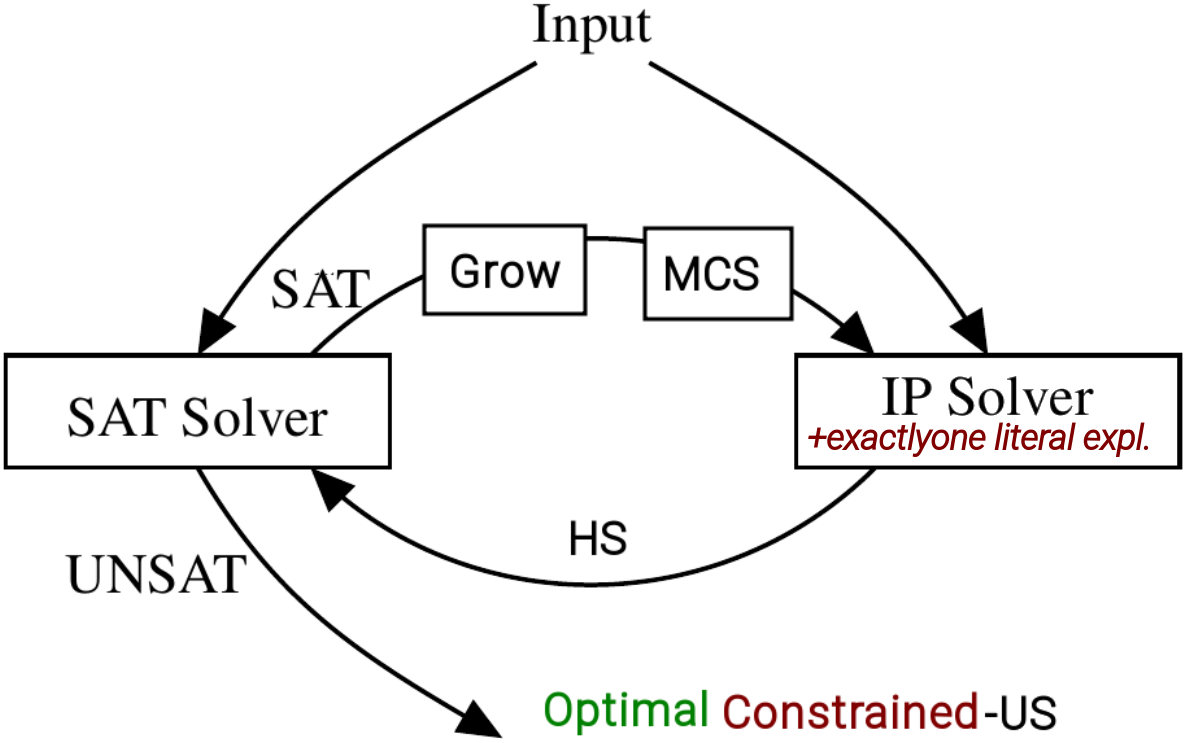
\includegraphics[width=\textwidth]{ihs_constrained.png}
		\end{figure}
	\end{minipage}
\vfill
\begin{figure}[h]
	
\includegraphics[width=\textwidth]{mus_to_ocus.png}
\end{figure}

\end{frame}

\begin{frame}{Incrementality}

	\begin{minipage}{0.59\textwidth}
		\begin{enumerate}
			\item Incremental \emph{OUSs}
\begin{itemize}
	\item Keep Satisfiable Subsets between OUS-calls
	\item Naïve OUS-restart $\rightarrow$ Keep 1 MIP solver warm per literal
	\begin{itemize}
		\item[$\implies$] No need to keep track of Satisfiable Subsets
	\end{itemize}

\end{itemize}
\item Optimizations
\begin{itemize}
			\item Keep track of cost for computed OUSs
	\item Sort the literals based on cost
\end{itemize}
\end{enumerate}
\end{minipage}
\begin{minipage}{0.4\textwidth}
	% TODO: ADD algorithm  one step !
	\begin{figure}
		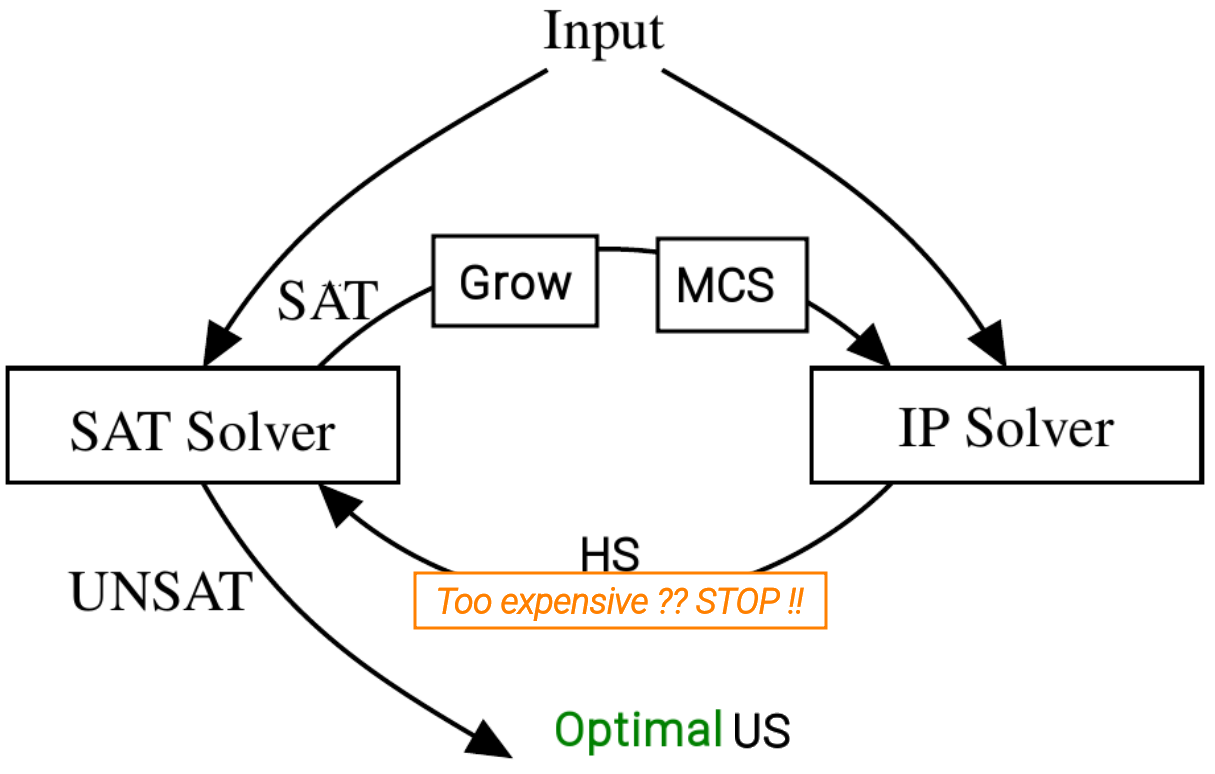
\includegraphics[width=\textwidth]{ihs_cost.png}
	\end{figure}
\end{minipage}\pause
\begin{figure}
	
\includegraphics[width=\textwidth]{mus_to_ous_i.png}
\end{figure}
\begin{enumerate}
	\setcounter{enumi}{1}
\item Incremnetal \emph{OCUS}	
\begin{itemize}
	\item Naïve OCUS-restart $\rightarrow$ Keep only 1 MIP solver warm
\end{itemize}	
\end{enumerate}
\begin{figure}
	
\includegraphics[width=\textwidth]{mus_to_ocus_i.png}
\end{figure}
\end{frame}

\begin{frame}{Contributions}
    \vfill
    In this paper, we 
    \vfill
    \begin{itemize}
        \item ... introduce (cost-)\textbf{\underline{O}ptimal} \underline{U}nsatisfiable \underline{S}ubsets (OUS) using the minimal hitting set duality
        \item ... analyze the structural constraints of the OUS explanations
        \item ... improve the efficiency of explanation sequence generation
    \end{itemize}
    \vfill
\end{frame}


\begin{frame}{Conclusion and Future work}

\end{frame}

\begin{frame}[allowframebreaks]
	\frametitle{References}
	\bibliographystyle{named}
	\bibliography{refs}
\end{frame}



\end{document}



